\documentclass[11pt]{beamer}
%\documentclass[11pt, aspectratio=169]{beamer}

\usepackage[utf8]{inputenc}
\usepackage[ngerman]{babel}
\usepackage{tikz}
\usetikzlibrary{shadows}
\usepackage{graphicx}
\usepackage[many]{tcolorbox}
\usepackage{moresize}

\usepackage{pifont}% http://ctan.org/pkg/pifont

\usepackage{listings}
\definecolor{deepblue}{rgb}{0,0,0.5}
\definecolor{deepred}{rgb}{0.6,0,0}
\definecolor{deepgreen}{rgb}{0,0.5,0}

%\newcommand\pythonstyle{\lstset{
\lstdefinestyle{myPython}{
		language=Python,
		basicstyle=\ssmall,
		numbers=left,
		breaklines=true,
		tabsize=2,
		frame=none,
		otherkeywords={self},             
		keywordstyle=\ttfamily\color{blue!90!black},
		keywords=[2]{True,False},
		keywords=[3]{ttk, row, column, sticky, fg, bg, font, lat, lon},
		keywordstyle={[2]\ttfamily\color{yellow!80!orange}},
		keywordstyle={[3]\ttfamily\color{red!80!orange}},
		emph={MyClass,__init__},          
		emphstyle=\ttfamily\color{red!80!black}, 
		stringstyle=\ttfamily\color{deepgreen},                        % Any extra options here
		showstringspaces=false            % 
%}}
}

\colorlet{punct}{red!60!black}
\definecolor{background}{HTML}{EEEEEE}
\definecolor{delim}{RGB}{20,105,176}
\colorlet{numb}{magenta!60!black}

\lstdefinelanguage{json}{
	basicstyle=\ssmall\ttfamily,
	numbers=left,
	numberstyle=\ssmall,
	stepnumber=1,
	numbersep=8pt,
	showstringspaces=false,
	breaklines=true,
	frame=lines,
	backgroundcolor=\color{background},
	literate=
	*{0}{{{\color{numb}0}}}{1}
	{1}{{{\color{numb}1}}}{1}
	{2}{{{\color{numb}2}}}{1}
	{3}{{{\color{numb}3}}}{1}
	{4}{{{\color{numb}4}}}{1}
	{5}{{{\color{numb}5}}}{1}
	{6}{{{\color{numb}6}}}{1}
	{7}{{{\color{numb}7}}}{1}
	{8}{{{\color{numb}8}}}{1}
	{9}{{{\color{numb}9}}}{1}
	{:}{{{\color{punct}{:}}}}{1}
	{,}{{{\color{punct}{,}}}}{1}
	{\{}{{{\color{delim}{\{}}}}{1}
	{\}}{{{\color{delim}{\}}}}}{1}
	{[}{{{\color{delim}{[}}}}{1}
	{]}{{{\color{delim}{]}}}}{1},
}


\newcommand{\cmark}{\ding{51}}%
\newcommand{\xmark}{\ding{55}}%

\usetheme{TuDo}
\begin{document}
	\author{Michael R. und Timon S.}
	\title{Smart Mirror}
	\subtitle{Proseminar: Raspberry Pi}
	\institute{TU Dortmund - Fakult\"at f\"ur Informatik}
	\date{\today}
	%\subject{}
	%\setbeamercovered{transparent}
	\titlegraphic{
		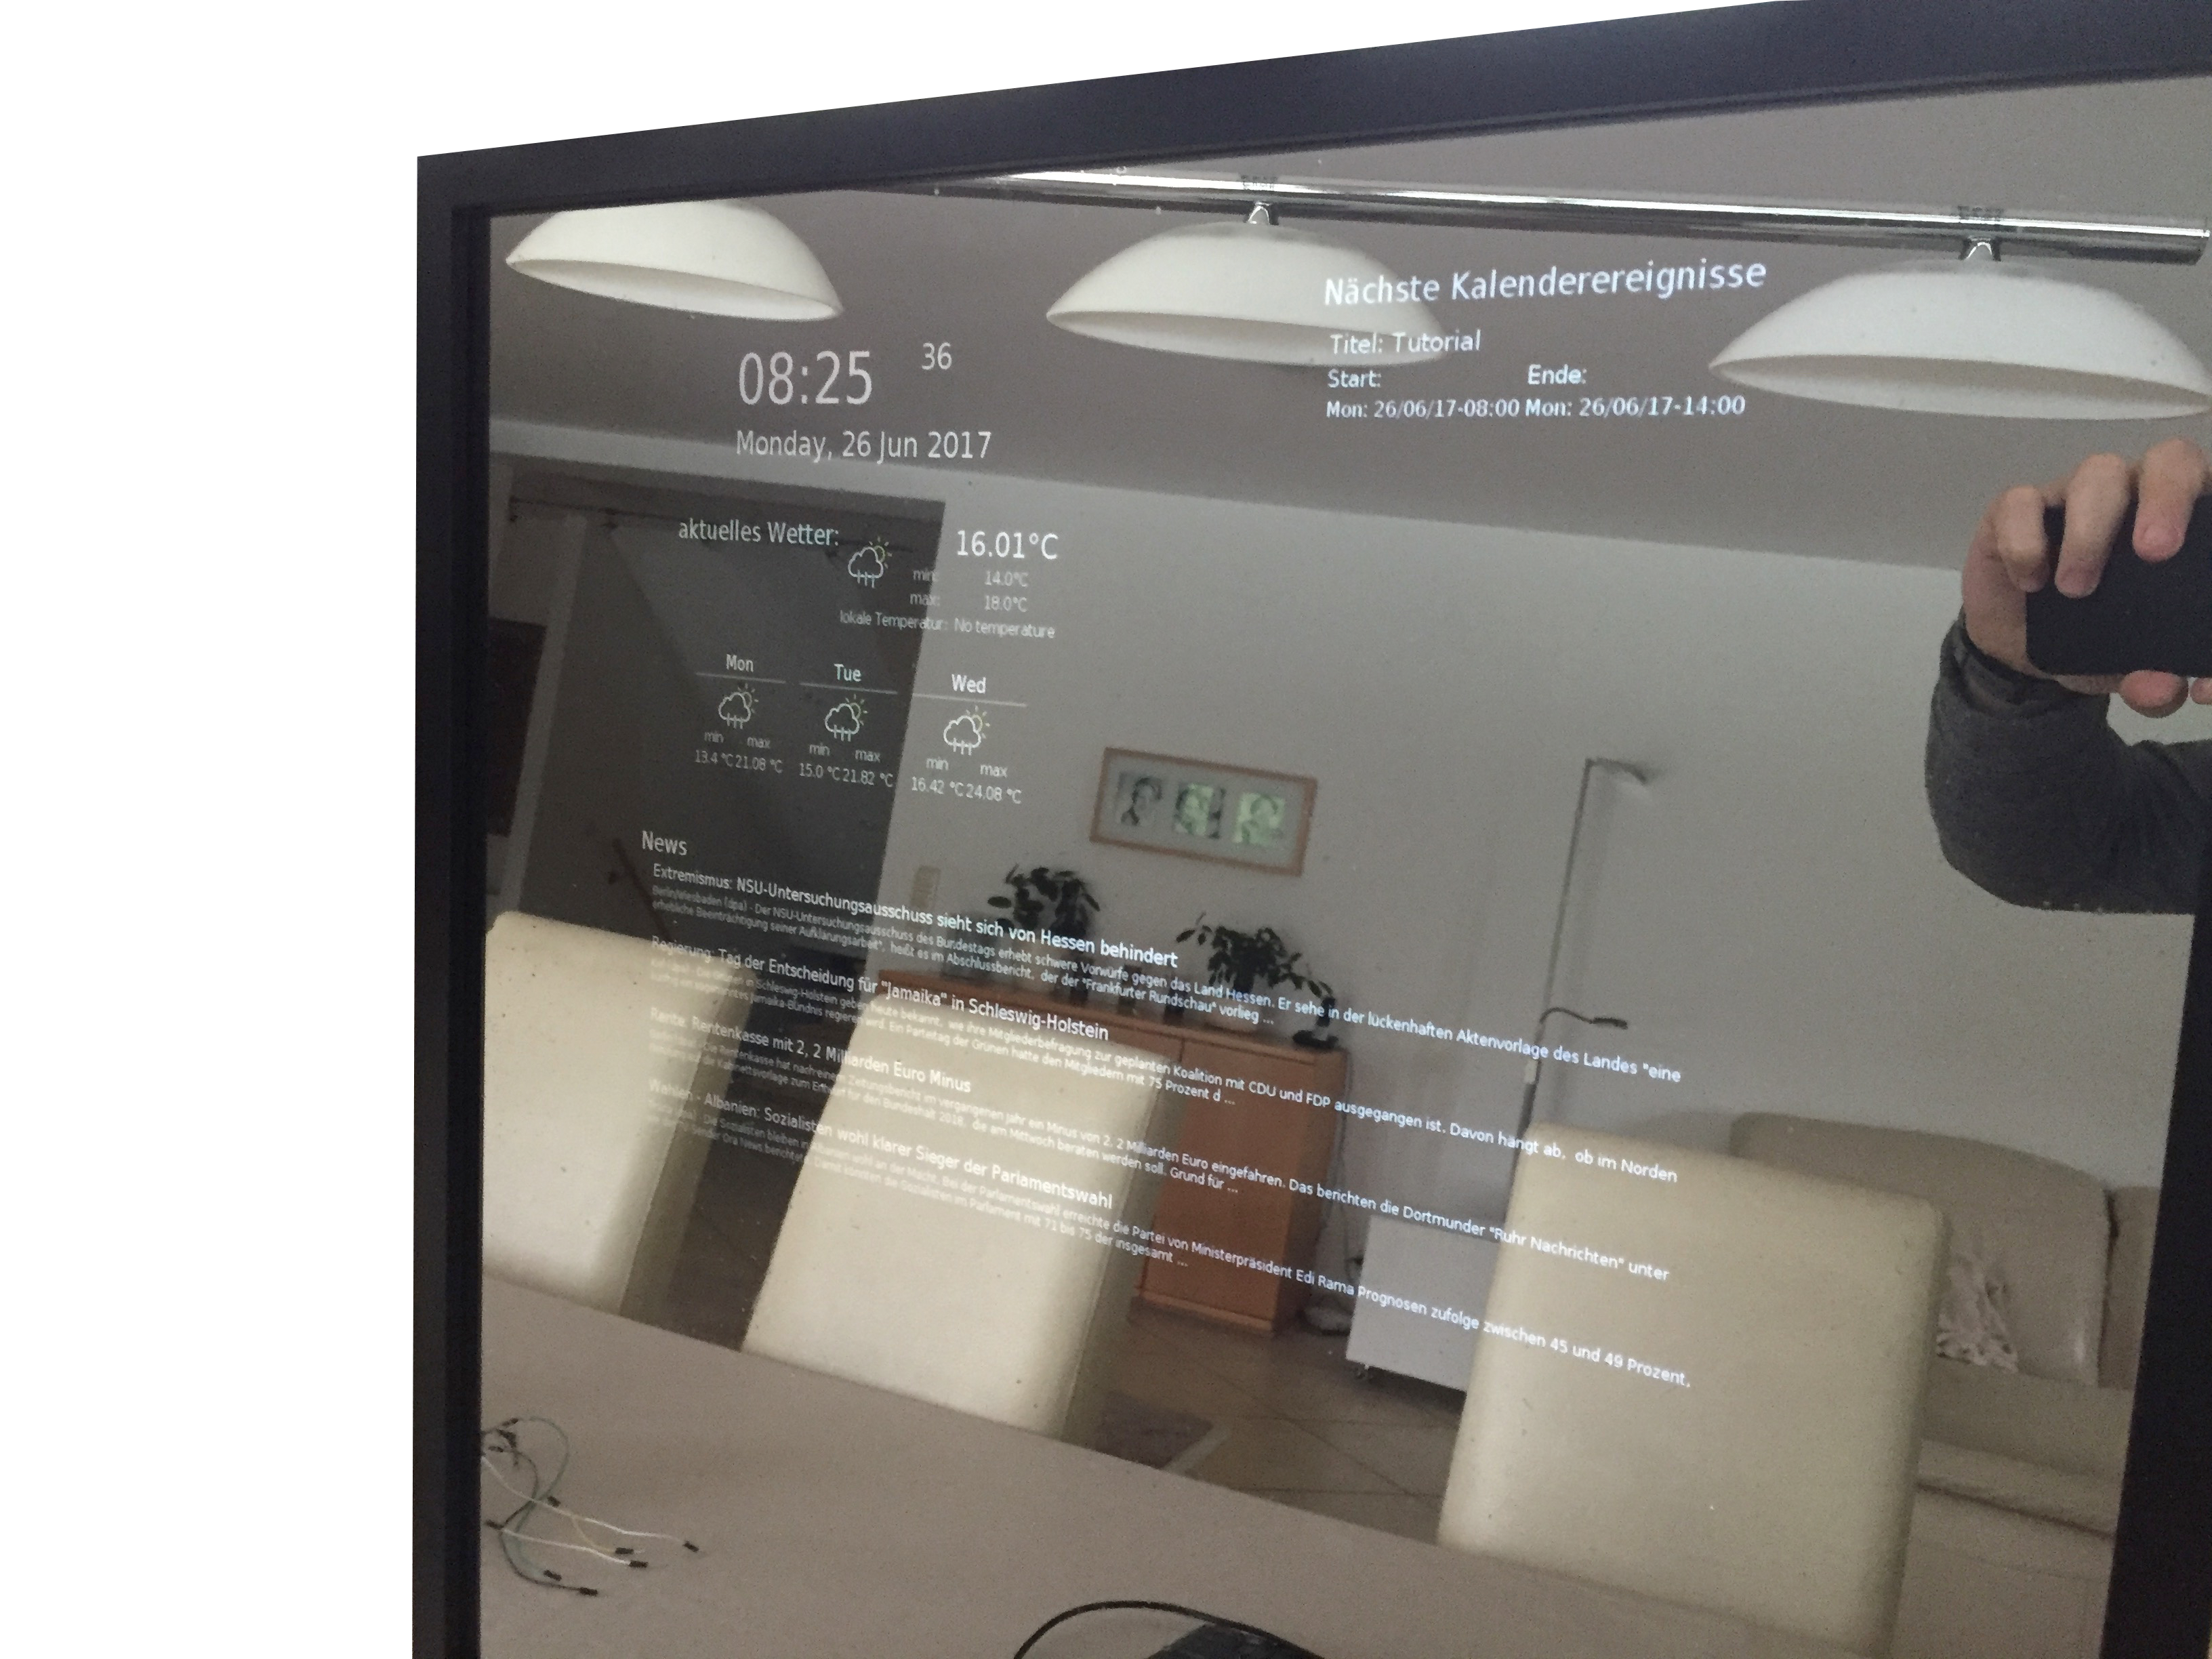
\includegraphics[width=0.35\paperwidth]{images/titlepage}
	}
	
	\begin{frame}
		\titlepage
	\end{frame}

	\begin{frame}
		\frametitle{Frage}
		\huge
		\begin{center}
			\vfill
			Vergisst du auch h\"aufig den Geburtstag deiner Großeltern?
			\vfill
		\end{center}
	\end{frame}

	\begin{frame}
		\frametitle{L\"osung}
		\begin{center}
			\Large
			So kann dir das nicht mehr passieren!
			\includegraphics[width = .7\paperwidth]{images/showcaseImage}
		\end{center}
	\end{frame}

	\begin{frame}
		\frametitle{Übersicht}
		\tableofcontents
	\end{frame}

	\section{Verteilung der Aufgaben}
	\begin{frame}
		\frametitle{Verteilung der Aufgaben}
	\end{frame}

	\section{technische Komponenten}
	\begin{frame}
		\frametitle{Hardwaregruppen}
		\begin{center}
			\Large{Aufteilung in Bereiche}
		\end{center}
		\begin{itemize}
		\item Ikearahmen 50x50 cm
		\item Displayeinheit
		\item Raspberry Pi und Sensoren
		\item Stromversorgung
		\end{itemize}
	\end{frame}
	
	\begin{frame}
		\frametitle{Rahmenaufbau}
	\end{frame}		

	\begin{frame}
		\frametitle{Technische Komponenten}
		\begin{itemize}
		\item 17 Zoll Monitor Format 4:3
		\item Netzteil für Monitor
		\item Display Controller HDMI zu IPEX-40Pin LVDS Kabel 
		\item Raspberry Pi 3
		\item Bewegungsmelder
		\item Temepraturfühler
		\item 5V Netzteil
		\item HDMI zu VGA Adapter
		\end{itemize}
	\end{frame}

	\subsection{Explosionsskizze}
	\begin{frame}
		\frametitle{Verteilungsdiagramm}
		\includegraphics[scale = 0.4]{images/smartMirrorExplosionsskizze.pdf}
	\end{frame}

	\section{UI}
	\begin{frame}
		\frametitle{Graphische Oberfl\"ache}
		\begin{center}
			\includegraphics[scale=0.3]{images/python+tkinter.png}
			\linebreak
			\includegraphics[scale=0.2]{images/grafOberflaeche.png}
		\end{center}
	\end{frame}
		
	\section{Programmierung}
	\subsection{Integration einer zwei-Schichten Architektur}
	\begin{frame}
		\frametitle{UML-Diagramm}
		\begin{center}
			\includegraphics[height=.7\paperheight]{images/umlDiagram}
		\end{center}
	\end{frame}

	\subsection{Aufbau eines Widgets}
\begin{frame}[fragile]
	\frametitle{Aufbau eines Widgets}
		
\begin{block}{Code}
%\pythonstyle
\lstinputlisting[frame=single, language=python, style=myPython, escapeinside={(*}{*)}]{codesnippets/frameExample.py}
\end{block}
\end{frame}

	\subsection{Von den Daten bis zur View}
	\begin{frame}
		\frametitle{Daten beziehen}
		\begin{center}
			\includegraphics[height=.55\paperheight]{images/sequenceDiagramGettingData}
		\end{center}
	\end{frame}

	\subsection{genutzte API's}
	\begin{frame}
		\frametitle{wichtigste API's}
		\begin{itemize}[<+->]
			\item pyowm
			\begin{itemize}[<.>]
				\item Wrapper um die OpenWeatherMap-Plattform
			\end{itemize}
			\item tkinter 
				\begin{itemize}[<.>]
					\item um die Oberfl\"ache zu designen
				\end{itemize}
			\item feedparser
				\begin{itemize}[<.>]
					\item vereinfacht den Zugriff auf JSON-Dokumente
				\end{itemize}
			\item requests
				\begin{itemize}[<.>]
					\item einfache Library (von Python integriert)
					\item bezieht Daten von entsprechender URL
					\item gibt die Daten als Raw-Values zur\"uck: JSON, HTML
				\end{itemize}
			\item apiclient, oauth2client
			\begin{itemize}[<.>]
				\item von Google bereitgestellte API's
				\item Zugang zu dem Google-Kalendar
				\item initiale Authorisierung der Anwendung mit OAuth2
			\end{itemize}
		\end{itemize}
	\end{frame}

	\subsection{JSON}
\begin{frame}[fragile]
		\frametitle{JSON}
		\begin{columns}
			\column{.45\paperwidth}
				\begin{itemize}
					\item JavaScript Object Notation
					\item Datenaustauschformat, welches einfach zu lesen ist
					\item unabh\"angig von Programmiersprachen
					\item Strukturen:
					\begin{itemize}
						\item Key-Value
						\item Liste
					\end{itemize}
				\end{itemize}
			\column{.45\paperwidth}
			\begin{block}{Beispiel}
				\lstinputlisting[language=json]{codesnippets/jsonExample.json}
			\end{block}
		\end{columns}
\end{frame}

\subsection{Nutzung von API's}
\begin{frame}[fragile]
		\frametitle{Nutzung von API's: pyowm}
		\begin{itemize}
			\item Zugriff auf Wetterdaten \"uber einen API-Key
			\item ruft spezifische URL mit dem API-Key auf
			\item bereitet die Daten als Wetter-Objekte auf
		\end{itemize}
\begin{block}{Code}
\lstinputlisting[frame=single, language=python, style=myPython]{codesnippets/apiaccessExample.py}
\end{block}
		\pause
		\begin{block}{Zusammenfassung}
			\begin{itemize}
				\item API's beziehen Daten vom Web
				\item API's erzeugen Objekte aus den Daten (meist JSON)
				\item Datenzugriff \"uber Attribute der Objekte
			\end{itemize}
		\end{block}
\end{frame}

	\section{Status}
	\begin{frame}
		\frametitle{Aktueller Status}
			\begin{columns}
				\column{.5\paperwidth}
					\begin{itemize}
						\item[\cmark] Oberfl\"ache designed
						\item[\cmark] ben\"otigte Libraries auf dem Pi installiert
						\item[\cmark] Spiegel zusammengebaut
						\item[\xmark] Display vermutlich defekt
						\item[\xmark] Temperatursensor auslesen
						\item[\xmark] Bewegungssensor angeschlossen
						\item Web-Oberfl\"ache f\"ur Datenerfassung
					\end{itemize}
				\column{.4\paperwidth}
					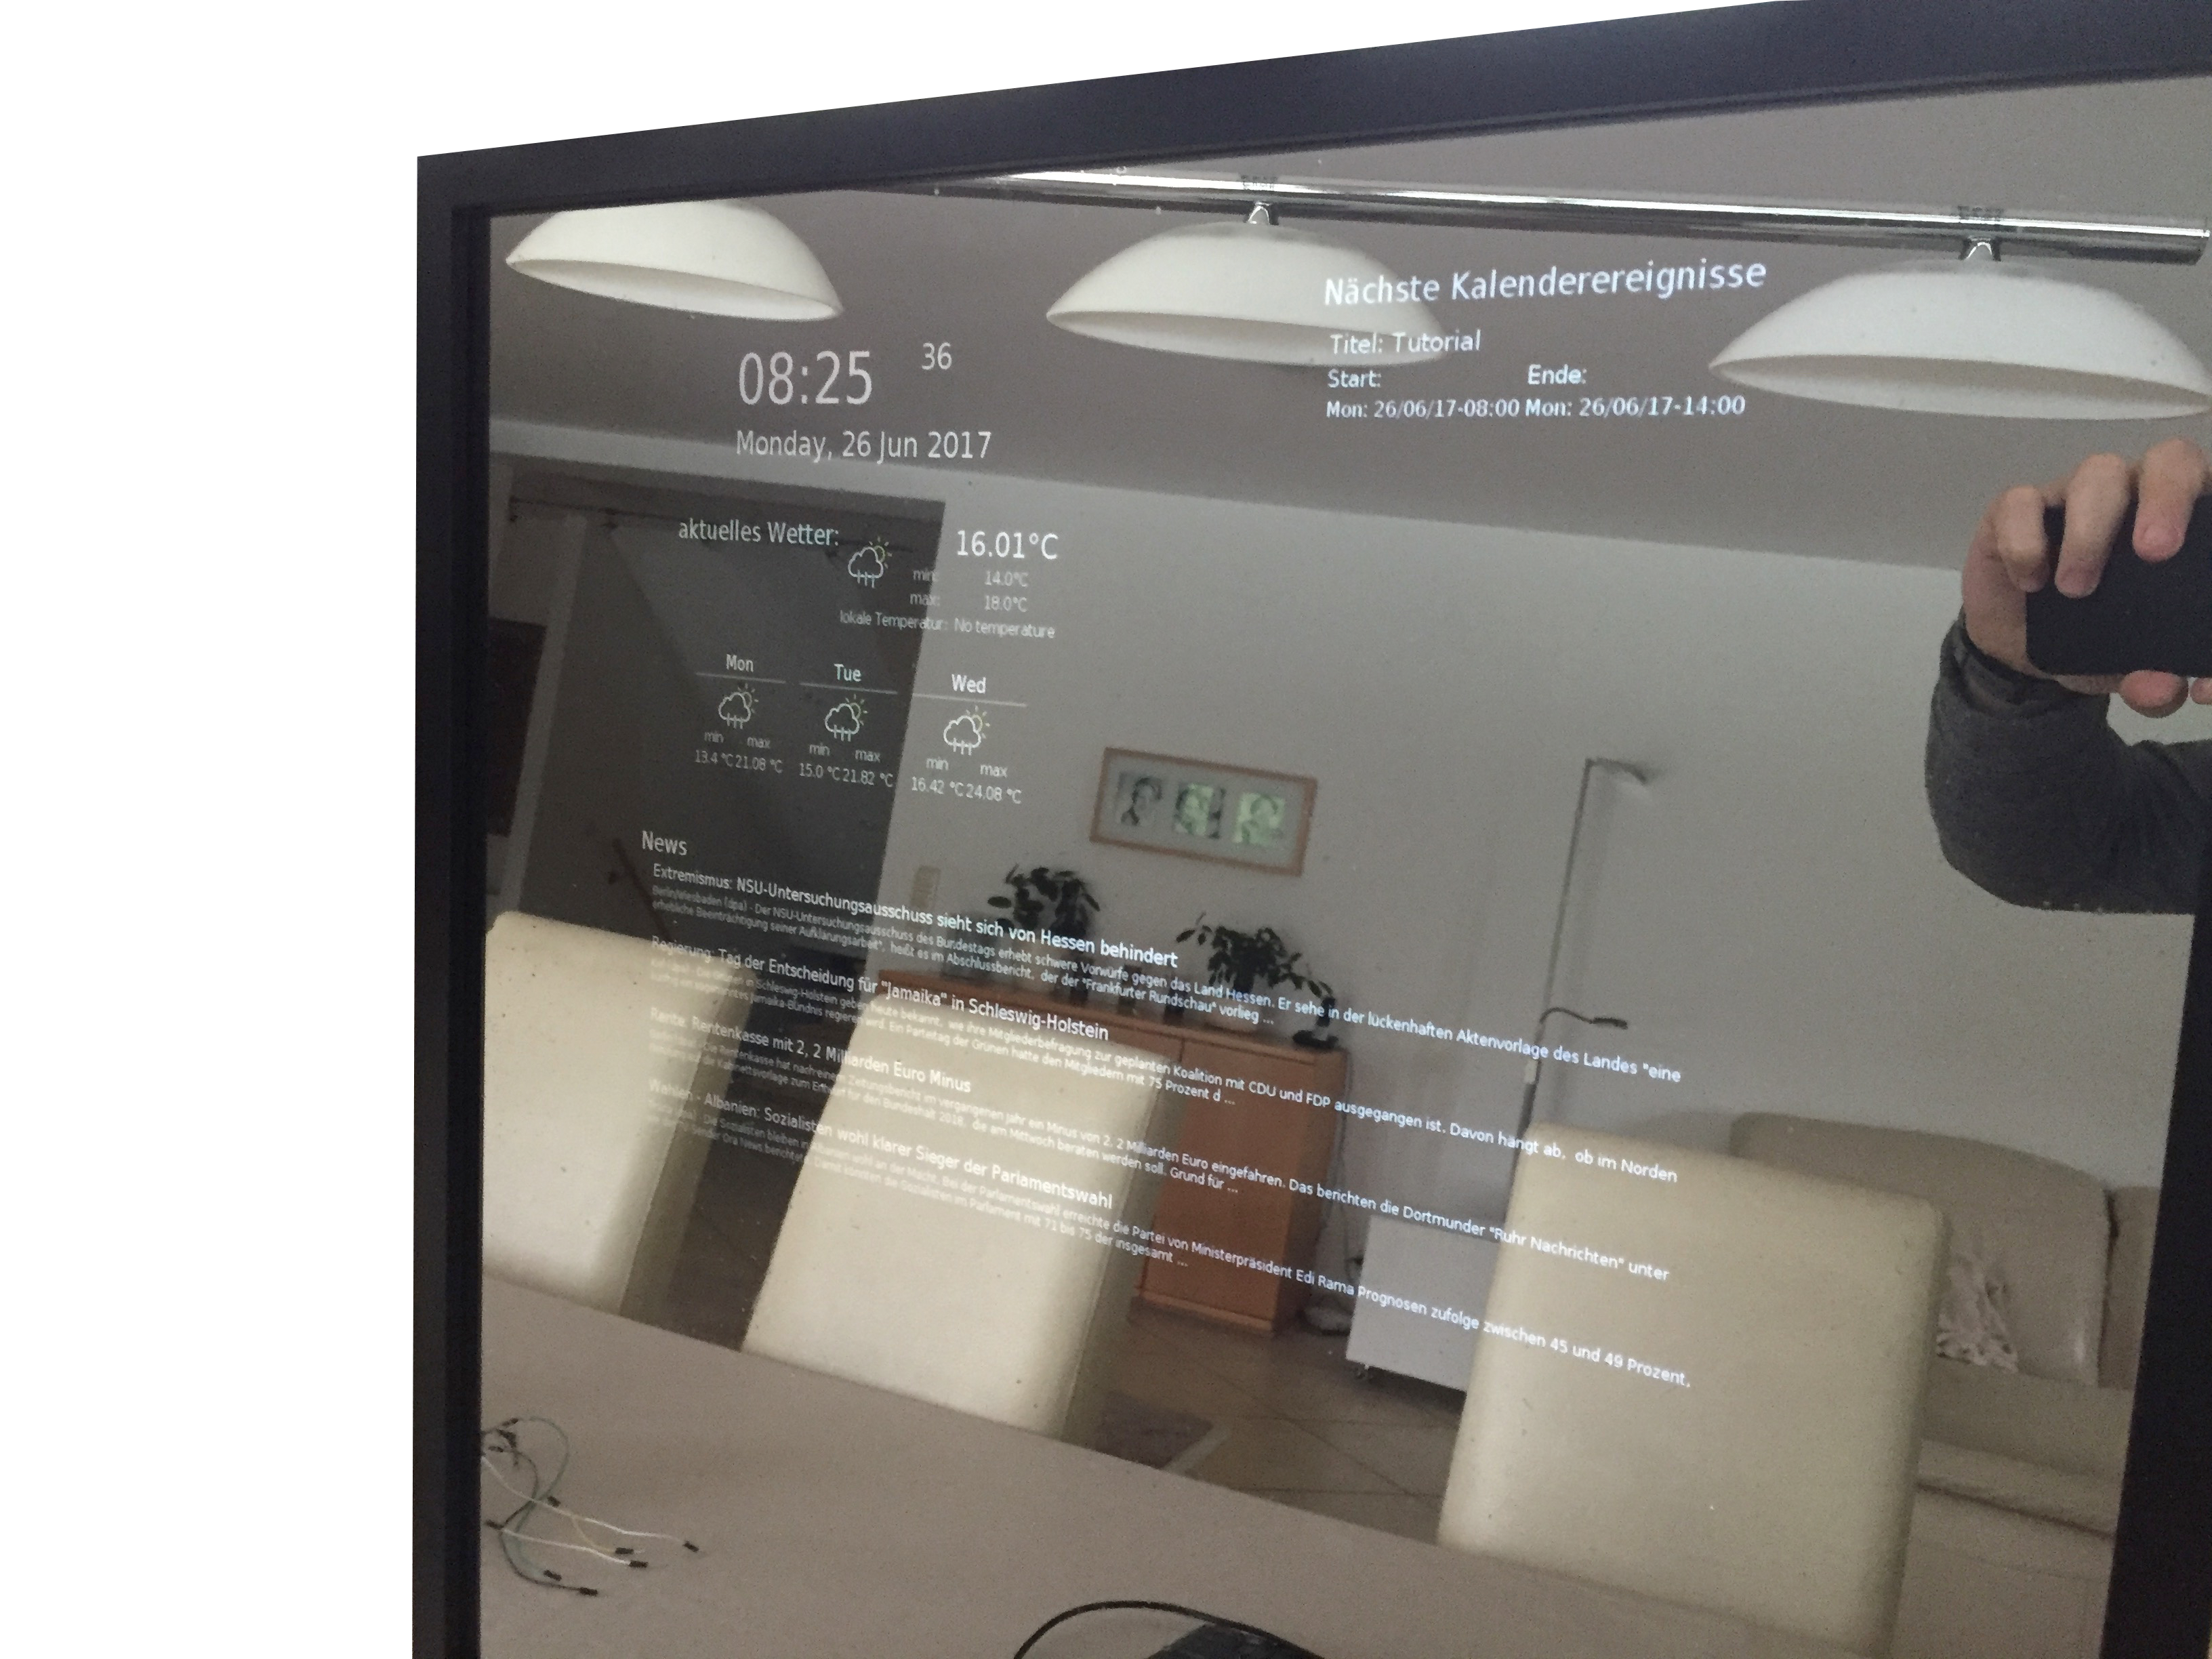
\includegraphics[width=.4\paperwidth]{images/titlepage}
			\end{columns}
	\end{frame}
	
	\section{Fazit}
	\begin{frame}
		\frametitle{Fazit}
		\centering
		\begin{block}{Spannende Aspekte}
			\begin{itemize}
				\item Absprache \"uber Teilprojekte
				\item Zusammenarbeit von Hard- und Software
				\item man muss im Team arbeiten
				\item am Ende komplett Lauff\"ahiges System in der Hand
			\end{itemize}
		\end{block}
		\pause
		\begin{block}{Wichtige Erfahrungen}
			\begin{itemize}
				\item Absprachen sind wichtig
				\item es l\"auft nicht immer alles so, wie gewollt
				\item Anwendungen f\"ur spezielle Hardware schreiben ist sinnvoll
			\end{itemize}
		\end{block}
	\end{frame}
\end{document}